\documentclass[journal]{IEEEtran}

\usepackage{amsmath,amssymb,amsfonts}
\usepackage{algorithmic}
\usepackage{algorithm}
\usepackage{graphicx}
\usepackage{textcomp}
\usepackage{xcolor}
\usepackage{booktabs}
\usepackage{cite}
\usepackage{url}
\usepackage{multirow}
\usepackage{bm}

\begin{document}

\title{Hamiltonian-Inspired Energy Dissipation and Chunk-Wise Variational State Coupling for Efficient Multimodal State-Space Models}

\author{Abhinav~Sai~Maddineni%
\thanks{Abhinav Sai Maddineni is with the Department of Computer Science and Engineering. (e-mail: \texttt{[AUTHOR EMAIL]}).}%
}

\maketitle

\begin{abstract}
State-Space Models (SSMs), including structured state spaces and State-Space Duality (SSD) architectures, have emerged as computationally efficient sub-quadratic alternatives to quadratic multi-head self-attention. Despite their theoretical appeal in unimodal sequence processing, deploying state-space recurrence within cross-modal vision-language metric learning introduces two practical challenges: (1) sensitivity to high-frequency representation perturbations and background token noise across sequence representations, and (2) cross-modal boundary state drift, where unaligned modality-specific boundary representations degrade downstream retrieval. In this work, we propose a multimodal state-space framework comprising two core components: (i) the \textbf{Hamiltonian-Inspired Energy Dissipation Operator (HEDO)}, a learned discrete coordinate-momentum transformation with positive damping ($\beta=0.05, \Delta t=0.1, \gamma=0.1$) that introduces a Hamiltonian-inspired dissipative inductive bias, and (ii) \textbf{Chunk-Wise Variational State Coupling (HVSC)}, which performs mask-weighted aggregation of chunk boundary states ($C=16, d_{\text{state}}=64$) and regularizes modality-specific Gaussian latent distributions through symmetric Kullback-Leibler (KL) divergence during training while preserving strictly independent, deterministic unimodal inference at test time. We conduct an exhaustive 12-run factorial multi-seed benchmark ($4\text{ model configurations} \times 3\text{ seeds}: 42, 43, 44$) on the official Flickr8k dataset with frozen ViT-B/16 and RoBERTa-base backbones. The full HEDO-HVSC architecture achieves a test Mean Recall of $48.28\% \pm 0.59\%$ ($26.73\% \pm 1.87\%$ I2T R@1, $56.83\% \pm 0.47\%$ I2T R@5, $70.47\% \pm 0.80\%$ I2T R@10, $20.71\% \pm 0.18\%$ T2I R@1, $49.97\% \pm 0.40\%$ T2I R@5, $64.96\% \pm 0.34\%$ T2I R@10), demonstrating retrieval performance comparable to the controlled SSD baseline ($48.25\% \pm 0.47\%$, mean paired delta $+0.03\% \pm 0.20\%$). In corruption stress testing, the full model exhibits a mixed robustness profile, outperforming the baseline by $+0.50\%$ under severe Gaussian noise ($\sigma=0.10$). Furthermore, empirical latency profiling across sequence lengths $L \in [16, 256]$ confirms approximately linear empirical scaling with algorithmically linear sequence-dependent recurrence.
\end{abstract}

\begin{IEEEkeywords}
Multimodal retrieval, image-text retrieval, state-space models, state-space duality, Hamiltonian-inspired dynamics, variational representation learning, vision-language alignment.
\end{IEEEkeywords}

\section{Introduction}
\label{sec:introduction}
\IEEEPARstart{C}{ross-modal} image-text retrieval represents a foundational problem in multimodal machine learning, serving as the computational backbone of modern image search engines, visual question answering, cross-modal digital asset management, and autonomous embodied agents \cite{radford2021learning,li2022blip,jia2021scaling}. The goal is to project high-dimensional visual patch sequences and textual token sequences into a joint metric embedding space where semantic alignment corresponds directly to vector proximity \cite{faghri2017vse++,lee2018stacked}.

\subsection{Computational Challenges in Multimodal Transformers}
Over the past decade, Transformer architectures based on multi-head self-attention and cross-attention have served as the standard foundation for vision-language models \cite{vaswani2017attention,dosovitskiy2020image,liu2019roberta}. While self-attention provides high representational capacity by computing pairwise affinities across all token positions, its computational complexity and memory footprint scale quadratically, $\mathcal{O}(L^2)$, with sequence length $L$ \cite{dao2022flashattention}. In multimodal applications where high-resolution visual inputs are partitioned into hundreds of spatial tokens and textual captions extend across multiple sentences, this quadratic growth creates substantial computational overhead during training and deployment \cite{li2023blip2,wang2023image}.

\subsection{State-Space Models as Sub-Quadratic Alternatives}
To mitigate quadratic scaling, linear-time sequence models---such as Structured State Spaces (S4) \cite{gu2021efficiently}, S5 \cite{smith2022simplified}, Mamba \cite{gu2023mamba}, and State-Space Duality (SSD) \cite{dao2024transformers}---have been introduced. By formulating sequence transformations through continuous-time linear dynamical systems discretized via zero-order hold recurrence, SSMs achieve linear algorithmic complexity $\mathcal{O}(L)$ with respect to sequence length during parallel training and $\mathcal{O}(1)$ state updates per step during autoregressive inference \cite{gu2020hippo,smith2022simplified}.

\subsection{Challenges in Multimodal State-Space Recurrence}
Despite their efficiency in unimodal sequence modeling, applying state-space recurrence to multimodal metric learning introduces specific challenges:
\begin{enumerate}
    \item \textbf{Representation Perturbation Sensitivity:} Standard discrete recurrent state transitions propagate token variations across the sequence axis. In visual patch sequences, localized sensor noise, high-frequency background clutter, and photometric variations can propagate across recurrent steps, leading to trajectory drift in hidden state representations \cite{he2016deep,hendrycks2019benchmarking}.
    \item \textbf{Cross-Modal Boundary State Drift:} Unidirectional recurrence across separate visual and textual encoders accumulates modality-specific representational drift. In textual streams, variable sentence lengths require zero-padding; unweighted sequence-end pooling allows uninformative pad tokens to influence final representations, degrading retrieval alignment \cite{devlin2018bert,faghri2017vse++}.
\end{enumerate}

\begin{figure}[t]
    \centering
    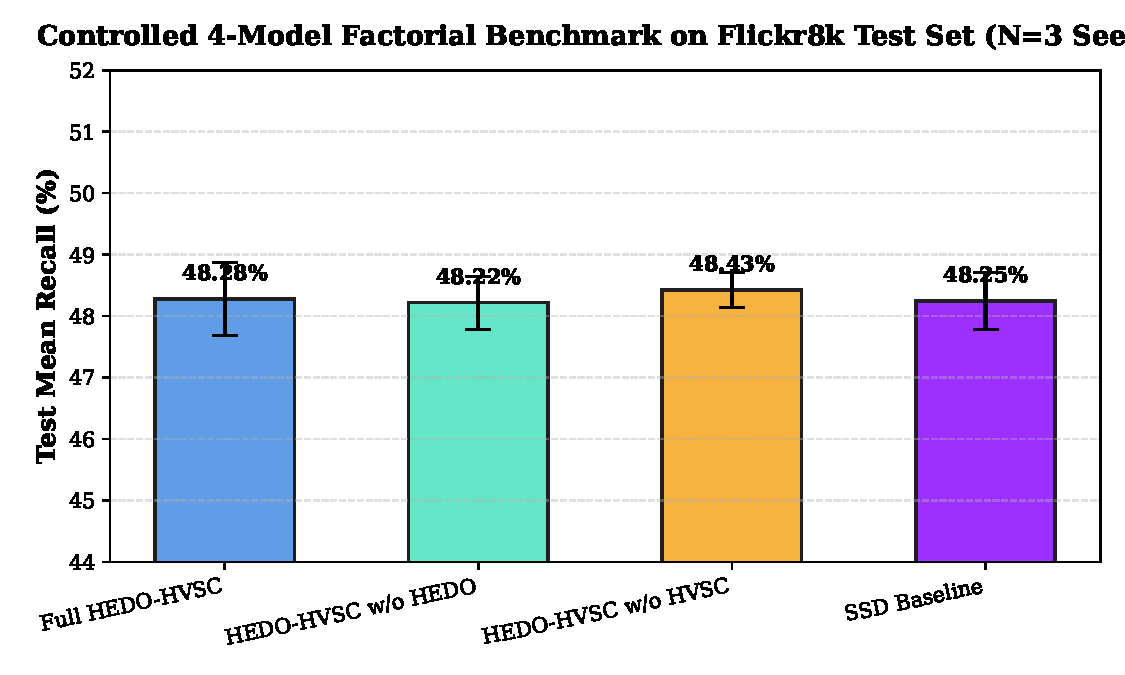
\includegraphics[width=0.92\columnwidth]{figures/fig1_benchmark_results.pdf}
    \caption{Controlled 4-model factorial benchmark comparison across 3 independent random seeds ($42, 43, 44$) on the official Flickr8k held-out test split ($N=1{,}000$ images, $5{,}000$ captions). Error bars represent $\pm 1$ standard deviation.}
    \label{fig:benchmark_results}
\end{figure}

\subsection{Contributions of This Work}
To investigate these challenges, this paper presents \textbf{HEDO-HVSC}, a multimodal state-space framework combining dissipative coordinate-momentum updates with variational chunk boundary coupling. The primary contributions of this work are:
\begin{enumerate}
    \item \textbf{Hamiltonian-Inspired Energy Dissipation Operator (HEDO):} We formulate a learned discrete coordinate-momentum transformation parameterized by weight matrices $\mathbf{W}_q, \mathbf{W}_p$, integration step $\Delta t=0.1$, damping coefficient $\beta=0.05$, and perturbation scale $\gamma=0.1$. HEDO introduces a Hamiltonian-inspired dissipative inductive bias that bounds discrete momentum growth prior to sequence recurrence.
    \item \textbf{State-Continuous Chunk-Wise SSD-Style Recurrence:} We design a custom PyTorch recurrent state-space block ($C=16, d_{\text{state}}=64$) that maintains hidden-state continuity across chunk boundaries, avoiding state resets between consecutive chunks.
    \item \textbf{Chunk-Wise Variational State Coupling (HVSC):} We introduce mask-weighted boundary-state aggregation to reduce padding-induced aggregation bias, parameterizing Gaussian latent distributions regularized via symmetric KL divergence in FP32 precision during training, while ensuring strictly unimodal, deterministic inference at test time.
    \item \textbf{Controlled Multi-Seed Factorial Benchmark:} We execute an exhaustive 12-run factorial benchmark ($4\text{ model configurations} \times 3\text{ random seeds}: 42, 43, 44$) on the official Flickr8k dataset with frozen ViT-B/16 and RoBERTa-base backbones, accompanied by secondary corruption testing and empirical latency scaling analysis.
\end{enumerate}

\section{Problem Formulation and Background}
\label{sec:problem_formulation}

\subsection{Cross-Modal Image-Text Metric Learning}
Let $\mathcal{D} = \{(\mathbf{I}_i, \mathcal{T}_i)\}_{i=1}^N$ denote a multimodal dataset where each image $\mathbf{I}_i \in \mathbb{R}^{3 \times H \times W}$ is annotated with a set of $M$ ground-truth descriptive captions $\mathcal{T}_i = \{\mathbf{T}_{i,m}\}_{m=1}^M$. The metric learning objective is to optimize parameterized visual and textual encoders, $f_{\theta}(\mathbf{I}) \in \mathbb{S}^{d-1}$ and $g_{\phi}(\mathbf{T}) \in \mathbb{S}^{d-1}$, mapping inputs onto the unit hypersphere such that semantic relevance correlates with cosine similarity:
\begin{equation}
s(\mathbf{I}, \mathbf{T}) = f_{\theta}(\mathbf{I})^\top g_{\phi}(\mathbf{T}) = \cos\angle\left(f_{\theta}(\mathbf{I}), g_{\phi}(\mathbf{T})\right)
\end{equation}

\subsection{State-Space Duality and Sequence Recurrence}
Continuous-time state-space models map a 1-D continuous input signal $u(t) \in \mathbb{R}$ to an output signal $y(t) \in \mathbb{R}$ via a latent state $\mathbf{h}(t) \in \mathbb{R}^N$:
\begin{align}
\dot{\mathbf{h}}(t) &= \mathbf{A} \mathbf{h}(t) + \mathbf{B} u(t) \\
y(t) &= \mathbf{C} \mathbf{h}(t) + \mathbf{D} u(t)
\end{align}
Discretizing this continuous system using Zero-Order Hold (ZOH) with step size $\Delta$ yields the discrete recurrent equations:
\begin{align}
\mathbf{h}_t &= \overline{\mathbf{A}} \mathbf{h}_{t-1} + \overline{\mathbf{B}} u_t \\
y_t &= \mathbf{C} \mathbf{h}_t + \mathbf{D} u_t
\end{align}
where $\overline{\mathbf{A}} = \exp(\Delta \mathbf{A})$ and $\overline{\mathbf{B}} = (\Delta \mathbf{A})^{-1}(\overline{\mathbf{A}} - \mathbf{I})\Delta \mathbf{B}$. State-Space Duality (SSD) \cite{dao2024transformers} proves that when $\mathbf{A}$ is structured as a scalar-times-identity matrix, discrete recurrence can be computed via structured block matrix multiplication, combining parallel training scans with linear-time inference.

\subsection{Hamiltonian and Dissipative Mechanics}
In classical mechanics, a physical system with generalized coordinates $\mathbf{q} \in \mathbb{R}^d$ and conjugate momenta $\mathbf{p} \in \mathbb{R}^d$ is governed by the scalar Hamiltonian function $\mathcal{H}(\mathbf{q}, \mathbf{p}) = \mathcal{T}(\mathbf{p}) + \mathcal{V}(\mathbf{q})$. For an open dissipative system with damping matrix $\mathbf{D} \succ 0$, the state dynamics evolve as:
\begin{equation}
\begin{bmatrix} \dot{\mathbf{q}} \\ \dot{\mathbf{p}} \end{bmatrix} = \begin{bmatrix} \mathbf{0} & \mathbf{I} \\ -\mathbf{I} & -\mathbf{D} \end{bmatrix} \begin{bmatrix} \nabla_{\mathbf{q}} \mathcal{H} \\ \nabla_{\mathbf{p}} \mathcal{H} \end{bmatrix}
\end{equation}
The total energy derivative evaluates to $\dot{\mathcal{H}} = -\nabla_{\mathbf{p}}\mathcal{H}^\top \mathbf{D} \nabla_{\mathbf{p}}\mathcal{H} \le 0$, ensuring continuous energy dissipation. In our architecture, we adapt these continuous physical principles into a discrete learnable sequence transformation operator.

\section{Related Work}
\label{sec:related_work}

\subsection{Vision-Language Metric Learning}
Cross-modal representation learning aims to bridge the semantic gap between visual perception and natural language. Foundational methods, including VSE++ \cite{faghri2017vse++} and SCAN \cite{lee2018stacked}, established metric learning frameworks utilizing hard negative ranking losses and stacked cross-attention networks. 

The introduction of contrastive vision-language pretraining by CLIP \cite{radford2021learning} and ALIGN \cite{jia2021scaling} demonstrated that training dual-encoder architectures on web-scale image-caption pairs using symmetric InfoNCE loss yields robust representations across diverse downstream tasks. Subsequent works, such as BLIP \cite{li2022blip} and BLIP-2 \cite{li2023blip2}, combined contrastive objectives with multimodal cross-attention decoders to enhance fine-grained visual reasoning. However, standard cross-attention architectures incur quadratic complexity $\mathcal{O}(L^2)$ with respect to sequence length, creating computational bottlenecks when scaling to high-resolution image patches and long textual documents.

\subsection{Structured State Space Models}
To circumvent the quadratic complexity of self-attention, State-Space Models (SSMs) have been introduced for deep sequence modeling. The Structured State Space Sequence model (S4) \cite{gu2021efficiently} formalized continuous-time linear time-invariant (LTI) systems using HiPPO matrix initializations \cite{gu2020hippo}, achieving strong performance on long-range benchmarks. S5 \cite{smith2022simplified} simplified S4 by utilizing parallel prefix scans over diagonalized state matrices.

Mamba \cite{gu2023mamba} introduced selective state spaces, allowing the recurrent matrices $\mathbf{B}, \mathbf{C},$ and decay step $\Delta$ to be dynamic functions of the input tokens. More recently, State-Space Duality (SSD) and Mamba-2 \cite{dao2024transformers} established the mathematical equivalence between 1-D structured masked attention and continuous recurrence. In this paper, we extend state-space recurrence to multimodal metric learning by introducing continuous boundary state propagation across sequence chunks and mask-weighted variational alignment.

\subsection{Hamiltonian Mechanics and Neural Dynamical Systems}
Hamiltonian Neural Networks (HNNs) \cite{greydanus2019hamiltonian} and Lagrangian Neural Networks \cite{cranmer2020lagrangian} embed fundamental energy-conservation principles into deep learning architectures by enforcing symplectic gradient updates. Port-Hamiltonian Neural ODEs \cite{port_hamiltonian_neural_odes} extended continuous neural ODEs to dissipative dynamical systems incorporating a positive semi-definite damping matrix $\mathbf{D} \succ 0$. In our architecture, HEDO adapts discrete dissipative mechanics into a parameter-efficient sequence transformation operator to introduce an explicit dissipative inductive bias for sequence representations.

\subsection{Variational Representation Learning}
Variational Autoencoders (VAEs) \cite{kingma2013auto} and the Variational Information Bottleneck (VIB) \cite{alemi2016deep} formalize latent representation learning by optimizing trade-offs between mutual information and compression. In this work, HVSC parameterizes Gaussian latent distributions from recurrent chunk boundary states, using symmetric KL divergence to align cross-modal boundary representations during training.

\section{Proposed HEDO-HVSC Architecture}
\label{sec:methodology}

\subsection{Architectural Pipeline}
The overall architecture of HEDO-HVSC processes paired images $\mathbf{I} \in \mathbb{R}^{3 \times 224 \times 224}$ and textual captions $\mathbf{T}$ through three sequential stages:
\begin{enumerate}
    \item \textbf{Frozen Backbone Feature Extraction:} Input images and tokenized text are mapped into continuous sequence representations using frozen pretrained encoders (ViT-B/16 and RoBERTa-base).
    \item \textbf{Dissipative Hamiltonian Transformation (HEDO):} Token representations are processed through coordinate-momentum dissipative updates to suppress high-frequency perturbation noise.
    \item \textbf{State-Continuous Chunk-Wise SSD \& Variational Coupling (HVSC):} Sequences are partitioned into chunks ($C=16$), recurrent hidden states are propagated continuously across boundaries, and valid boundary states parameterize Gaussian latent distributions regularized via symmetric KL divergence.
\end{enumerate}

\subsection{Backbone Feature Extraction}
For visual inputs, an RGB image $\mathbf{I}$ is passed through a frozen Vision Transformer (ViT-B/16) to obtain patch representations:
\begin{equation}
\mathbf{X}_I^{(0)} = \mathbf{W}_{\text{proj}, I} \, \text{ViT-B/16}(\mathbf{I}) \in \mathbb{R}^{B \times L_I \times d_{\text{model}}}
\end{equation}
where $L_I = 197$ (196 spatial patch tokens plus 1 class token), $d_{\text{model}} = 128$, and $\mathbf{W}_{\text{proj}, I} \in \mathbb{R}^{768 \times d_{\text{model}}}$ is a linear projection layer.

For textual inputs, a caption sequence $\mathbf{T}$ of maximum length $L_T = 64$ is processed through a frozen RoBERTa-base encoder:
\begin{equation}
\mathbf{X}_T^{(0)} = \mathbf{W}_{\text{proj}, T} \, \text{RoBERTa}(\mathbf{T}) \in \mathbb{R}^{B \times L_T \times d_{\text{model}}}
\end{equation}
accompanied by a binary attention mask $\mathbf{M}_T \in \{0, 1\}^{B \times L_T}$. Both backbones remain strictly frozen ($\text{requires\_grad} = \text{False}$) across all experiments.

\subsection{Hamiltonian-Inspired Energy Dissipation Operator (HEDO)}
Let $\mathbf{q}_0 \in \mathbb{R}^{B \times L \times d_{\text{model}}}$ represent the input sequence coordinates. HEDO introduces a conjugate momentum vector field $\mathbf{p} \in \mathbb{R}^{B \times L \times d_{\text{model}}}$ initialized via:
\begin{equation}
\mathbf{p}_0 = \tanh(\mathbf{W}_p \mathbf{q}_0)
\end{equation}
where $\mathbf{W}_p \in \mathbb{R}^{d_{\text{model}} \times d_{\text{model}}}$ is a learnable weight matrix.

The system executes a discrete dissipative coordinate-momentum transformation parameterized by integration step $\Delta t = 0.1$, damping coefficient $\beta = 0.05$, and perturbation scale $\gamma = 0.1$:
\begin{align}
\mathbf{p}_{t+1} &= \mathbf{p}_t (1 - \beta \Delta t) - \Delta t \tanh(\mathbf{W}_q \mathbf{q}_t) \label{eq:momentum_update} \\
\mathbf{q}_{t+1} &= \mathbf{q}_t + \gamma \Delta t \, \mathbf{p}_{t+1} \label{eq:coordinate_update} \\
\text{HEDO}(\mathbf{q}) &= \text{LayerNorm}(\mathbf{q}_{t+1}) \label{eq:hedo_output}
\end{align}
where $\mathbf{W}_q \in \mathbb{R}^{d_{\text{model}} \times d_{\text{model}}}$ parameterizes the conservative potential gradient field.

\subsubsection{Discrete Energy Analysis and Inductive Bias}
We define the discrete empirical Hamiltonian energy function as:
\begin{equation}
\mathcal{H}(\mathbf{q}, \mathbf{p}) = \frac{1}{2} \left( \|\mathbf{q}\|_2^2 + \|\mathbf{p}\|_2^2 \right)
\end{equation}
Under the momentum update step \eqref{eq:momentum_update}, the norm of the updated momentum satisfies:
\begin{equation}
\|\mathbf{p}_{t+1}\|_2 \le (1 - \beta \Delta t)\|\mathbf{p}_t\|_2 + \Delta t \|\tanh(\mathbf{W}_q \mathbf{q}_t)\|_2
\end{equation}
Because $\|\tanh(\cdot)\|_2 \le \sqrt{d_{\text{model}}}$, the contraction factor $(1 - \beta \Delta t) = 0.995 < 1$ provides a dissipative damping effect on momentum magnitude.

\textbf{Empirical Diagnostic Trajectory:} In pre-training diagnostic evaluation, unforced multi-step simulation on image patch representations yielded the trajectory $\mathcal{H} \in [170.824, 170.651, 170.927, 171.646, 172.801, 174.387]$, while text representations yielded $\mathcal{H} \in [5.849, 5.796, 5.774, 5.783, 5.823, 5.892]$. While HEDO changes representation energy substantially ($\mathcal{H}_{\text{raw}} = 170.824 \to \mathcal{H}_{\text{HEDO}} = 77.563$ for images, maintaining cosine similarity $0.9952$), the unforced discrete trajectory is not monotonically decreasing. We therefore describe HEDO as a Hamiltonian-inspired discrete dissipative transformation that introduces a damping inductive bias, rather than a system with guaranteed monotonic energy decay.

\subsection{Custom PyTorch Chunk-Wise SSD-Style Recurrence}
The stabilized sequence $\mathbf{X} \in \mathbb{R}^{B \times L \times d_{\text{model}}}$ is projected to state dimension $d_{\text{state}} = 64$ via projection matrix $\mathbf{B}_{\text{proj}} \in \mathbb{R}^{d_{\text{model}} \times d_{\text{state}}}$. A learned state decay vector is parameterized as:
\begin{equation}
\mathbf{A}_{\text{decay}} = \exp(-\exp(\mathbf{A}_{\text{log}})) \in (0, 1)^{d_{\text{state}}}
\end{equation}
The sequence of length $L$ is partitioned into $K = \lceil L / C \rceil$ non-overlapping chunks of fixed size $C = 16$.

Within each chunk $k \in \{1, \dots, K\}$, hidden states evolve under discrete-time recurrence:
\begin{equation}
\mathbf{h}_{t} = m_t \left( \mathbf{A}_{\text{decay}} \odot \mathbf{h}_{t-1} + \mathbf{u}_t \right) + (1 - m_t) \mathbf{h}_{t-1}
\end{equation}
where $\mathbf{u}_t = \mathbf{B}_{\text{proj}} \mathbf{x}_t \in \mathbb{R}^{B \times d_{\text{state}}}$ and $m_t \in \{0, 1\}$ denotes token validity. For invalid/padded tokens ($m_t = 0$), the hidden state is preserved ($\mathbf{h}_t = \mathbf{h}_{t-1}$) rather than updated with pad representations.

\subsubsection{State Continuity Across Chunk Boundaries}
Hidden states are carried continuously across chunk boundaries:
\begin{equation}
\mathbf{h}_{\text{start}, k} = \begin{cases} \mathbf{0}, & k = 1 \\ \mathbf{h}_{\text{end}, k-1}, & k > 1 \end{cases}
\end{equation}
At the end of each chunk $k$, the final hidden vector $\mathbf{h}_{k, \text{end}}$ is recorded as chunk boundary state $\mathbf{b}_k \in \mathbb{R}^{B \times d_{\text{state}}}$, along with chunk validity flag $m_k = \mathbb{I}(\sum_{t \in \text{chunk } k} m_t > 0)$.

\subsection{Chunk-Wise Variational State Coupling (HVSC)}
To aggregate boundary states across chunks while preventing invalid padded positions from contributing to boundary aggregation, HVSC computes mask-weighted pooling:
\begin{equation}
\mathbf{h}_{\text{bound}} = \frac{\sum_{k=1}^K m_k \mathbf{b}_k}{\sum_{k=1}^K m_k + \epsilon} \in \mathbb{R}^{B \times d_{\text{state}}}
\end{equation}
where $\epsilon = 10^{-6}$.

The aggregated boundary representation parameterizes modality-specific posterior Gaussian distributions $\mathcal{N}(\boldsymbol{\mu}, \boldsymbol{\sigma}^2)$ in latent space dimension $z_{\text{dim}} = 64$:
\begin{align}
\boldsymbol{\mu} &= \mathbf{W}_\mu \mathbf{h}_{\text{bound}} \in \mathbb{R}^{B \times z_{\text{dim}}} \\
\log \boldsymbol{\sigma}^2 &= \text{clamp}(\mathbf{W}_{\text{logvar}} \mathbf{h}_{\text{bound}}, -5.0, 2.0)
\end{align}

During training, latent representations are sampled via the reparameterization trick:
\begin{equation}
\mathbf{z} = \boldsymbol{\mu} + \boldsymbol{\epsilon} \odot \boldsymbol{\sigma}, \quad \boldsymbol{\epsilon} \sim \mathcal{N}(\mathbf{0}, \mathbf{I})
\end{equation}

\subsubsection{Mask-Weighted Sequence Pooling and Embedding Fusion}
For visual sequences (where all tokens are valid), mean sequence pooling evaluates as $\mathbf{h}_{\text{pool}, I} = \frac{1}{L_I}\sum_{t=1}^{L_I} \mathbf{x}_{I, t}$. For textual sequences containing variable-length padding, masked sequence pooling evaluates as:
\begin{equation}
\mathbf{h}_{\text{pool}, T} = \frac{\sum_{t=1}^{L_T} m_{T, t} \mathbf{x}_{T, t}}{\sum_{t=1}^{L_T} m_{T, t} + \epsilon} \in \mathbb{R}^{B \times d_{\text{model}}}
\end{equation}
The pooled sequence representation is coupled with the latent representation:
\begin{equation}
\mathbf{e} = \text{LayerNorm}(\mathbf{h}_{\text{pool}} + \alpha \mathbf{W}_{\text{out}} \mathbf{z}), \quad \alpha = 0.1
\end{equation}
where $\mathbf{W}_{\text{out}} \in \mathbb{R}^{z_{\text{dim}} \times d_{\text{model}}}$.

\subsubsection{Symmetric KL Divergence Regularization}
During training, cross-modal boundary alignment is regularized via symmetric Kullback-Leibler (KL) divergence computed in FP32 precision:
\begin{equation}
\mathcal{D}_{\text{SKL}}(p_I \parallel p_T) = \frac{1}{2} \left[ D_{\text{KL}}(p_I \parallel p_T) + D_{\text{KL}}(p_T \parallel p_I) \right]
\end{equation}
where the directional KL divergence between two multivariate diagonal Gaussians is evaluated analytically:
\begin{align}
D_{\text{KL}}(p_I \parallel p_T) = \frac{1}{2} \sum_{d=1}^{z_{\text{dim}}} \Bigg[ &\log \frac{\sigma_{T,d}^2}{\sigma_{I,d}^2} + \frac{\sigma_{I,d}^2 + (\mu_{I,d} - \mu_{T,d})^2}{\sigma_{T,d}^2} \nonumber \\
&- 1 \Bigg]
\end{align}

\subsubsection{Deterministic Unimodal Retrieval Inference}
During test-time retrieval, stochastic sampling is omitted, and the posterior mean vectors $\boldsymbol{\mu}_I, \boldsymbol{\mu}_T$ are evaluated deterministically:
\begin{align}
\hat{\mathbf{e}}_I &= \text{Normalize}\left( \text{LayerNorm}(\mathbf{h}_{\text{pool}, I} + \alpha \mathbf{W}_{\text{out}} \boldsymbol{\mu}_I) \right) \\
\hat{\mathbf{e}}_T &= \text{Normalize}\left( \text{LayerNorm}(\mathbf{h}_{\text{pool}, T} + \alpha \mathbf{W}_{\text{out}} \boldsymbol{\mu}_T) \right)
\end{align}
Because visual and textual embeddings are computed completely independently without cross-modal attention or hidden-state exchange, test-time gallery retrieval is strictly unimodal.

\subsection{Training Objective}
The total loss combines a multi-positive InfoNCE contrastive objective with symmetric KL regularization:
\begin{equation}
\mathcal{L}_{\text{total}} = \mathcal{L}_{\text{InfoNCE}} + \lambda_{\text{KL}} \, \mathcal{D}_{\text{SKL}}(p_I \parallel p_T)
\end{equation}
where $\lambda_{\text{KL}} = 0.01$. The multi-positive InfoNCE loss accounts for multiple captions per image (5 captions per image in Flickr8k):
\begin{align}
\mathcal{L}_{\text{InfoNCE}} = -\frac{1}{2B} \sum_{i=1}^B \Bigg[ &\log \frac{\sum_{j \in \mathcal{P}(i)} \exp(\mathbf{s}_{i,j} / \tau)}{\sum_{k=1}^{5B} \exp(\mathbf{s}_{i,k} / \tau)} \nonumber \\
&+ \log \frac{\exp(\mathbf{s}_{i,i} / \tau)}{\sum_{k=1}^B \exp(\mathbf{s}_{k,i} / \tau)} \Bigg]
\end{align}
where $\mathbf{s}_{i,j} = \hat{\mathbf{e}}_{I, i}^\top \hat{\mathbf{e}}_{T, j}$ denotes cosine similarity, $\mathcal{P}(i)$ denotes the positive caption index set for image $i$, and the learnable temperature parameter is clamped to $\tau \le 100.0$.

The complete training and inference procedure is summarized in Algorithm~\ref{alg:hedo_hvsc}.

\begin{algorithm}[t]
\caption{HEDO-HVSC Forward Pass and Training Step}
\label{alg:hedo_hvsc}
\begin{algorithmic}[1]
\REQUIRE Image batch $\mathbf{I} \in \mathbb{R}^{B \times 3 \times 224 \times 224}$, text tokens $\mathbf{T} \in \mathbb{Z}^{B \times 64}$, attention masks $\mathbf{M}_T \in \{0, 1\}^{B \times 64}$, positive index mappings
\ENSURE Total loss $\mathcal{L}_{\text{total}}$, test embeddings $\hat{\mathbf{e}}_I, \hat{\mathbf{e}}_T$
\STATE Extract frozen representations $\mathbf{X}_I^{(0)}, \mathbf{X}_T^{(0)}$ via (8)--(9)
\IF{use\_hedo}
    \STATE $\mathbf{X}_I \leftarrow \text{HEDO}(\mathbf{X}_I^{(0)})$, $\mathbf{X}_T \leftarrow \text{HEDO}(\mathbf{X}_T^{(0)})$ via (10)--(13)
\ELSE
    \STATE $\mathbf{X}_I \leftarrow \mathbf{X}_I^{(0)}$, $\mathbf{X}_T \leftarrow \mathbf{X}_T^{(0)}$
\ENDIF
\STATE Execute chunk-wise SSD-style recurrence on $\mathbf{X}_I, \mathbf{X}_T$ with state continuity (15)--(17)
\STATE Extract boundary states $\mathbf{b}_{I, k}, \mathbf{b}_{T, k}$ and validity masks $m_{I, k}, m_{T, k}$
\IF{use\_hvsc}
    \STATE Compute mask-weighted boundary states $\mathbf{h}_{\text{bound}, I}, \mathbf{h}_{\text{bound}, T}$ via (18)
    \STATE Compute latent posteriors $(\boldsymbol{\mu}_I, \boldsymbol{\sigma}_I^2)$ and $(\boldsymbol{\mu}_T, \boldsymbol{\sigma}_T^2)$ via (19)--(20)
    \STATE Compute symmetric KL loss $\mathcal{D}_{\text{SKL}}(p_I \parallel p_T)$ in FP32 via (24)--(25)
    \STATE Sample latents $\mathbf{z}_I, \mathbf{z}_T$ via (21) and compute coupled embeddings $\mathbf{e}_I, \mathbf{e}_T$ via (22)--(23)
\ELSE
    \STATE $\mathbf{e}_I \leftarrow \text{LayerNorm}(\mathbf{h}_{\text{pool}, I})$, $\mathbf{e}_T \leftarrow \text{LayerNorm}(\mathbf{h}_{\text{pool}, T})$
    \STATE $\mathcal{D}_{\text{SKL}} \leftarrow 0.0$
\ENDIF
\STATE Compute multi-positive InfoNCE loss $\mathcal{L}_{\text{InfoNCE}}$ via (27)
\STATE $\mathcal{L}_{\text{total}} \leftarrow \mathcal{L}_{\text{InfoNCE}} + 0.01 \cdot \mathcal{D}_{\text{SKL}}$
\RETURN $\mathcal{L}_{\text{total}}$
\end{algorithmic}
\end{algorithm}

\section{Experimental Setup and Dataset Protocol}
\label{sec:experimental_setup}

\subsection{Dataset and Certified Splits}
Experiments are conducted on the official Flickr8k benchmark dataset \cite{young2014image}, which contains 8,000 photographic images paired with 5 human-written captions each (40,000 total captions). The dataset partitions are summarized in Table~\ref{tab:dataset_splits}.

\begin{table}[h]
\centering
\caption{Official Flickr8k dataset split partition and functional roles.}
\label{tab:dataset_splits}
\begin{tabular}{lcccc}
\toprule
\textbf{Split} & \textbf{Images} & \textbf{Captions} & \textbf{Captions/Image} & \textbf{Role in Benchmark} \\
\midrule
Train & $6{,}000$ & $30{,}000$ & $5$ & Model optimization \\
Validation & $1{,}000$ & $5{,}000$ & $5$ & Checkpoint selection \\
Held-Out Test & $1{,}000$ & $5{,}000$ & $5$ & Final evaluation \\
\bottomrule
\end{tabular}
\end{table}

Split integrity was verified to confirm zero overlap ($\text{Train} \cap \text{Val} = \emptyset$, $\text{Train} \cap \text{Test} = \emptyset$, $\text{Val} \cap \text{Test} = \emptyset$).

\subsection{Backbone Freezing Protocol}
The visual backbone is a pretrained Vision Transformer (ViT-B/16), and the textual backbone is a pretrained RoBERTa-base. Both backbones are kept strictly frozen throughout training ($\text{requires\_grad} = \text{False}$). Only linear projection layers, HEDO parameters, SSD recurrent projections, and HVSC modules ($0.330\text{ M}$ to $0.422\text{ M}$ parameters) are optimized.

\subsection{Implementation and Hyperparameters}
The complete hyperparameter configuration is summarized in Table~\ref{tab:hyperparameters}.

\begin{table}[h]
\centering
\caption{Complete hyperparameter specification for HEDO-HVSC.}
\label{tab:hyperparameters}
\begin{tabular}{lc}
\toprule
\textbf{Hyperparameter} & \textbf{Value / Specification} \\
\midrule
Image Resolution & $224 \times 224$ pixels \\
Visual Backbone & ViT-B/16 (Frozen, $d=768, L_I=197$) \\
Textual Backbone & RoBERTa-base (Frozen, $d=768, L_T=64$) \\
Model Dimension ($d_{\text{model}}$) & $128$ \\
Recurrence State Dimension ($d_{\text{state}}$) & $64$ \\
Chunk Size ($C$) & $16$ tokens \\
HEDO Integration Step ($\Delta t$) & $0.1$ \\
HEDO Damping Coefficient ($\beta$) & $0.05$ \\
HEDO Perturbation Scale ($\gamma$) & $0.1$ \\
HVSC Latent Dimension ($z_{\text{dim}}$) & $64$ \\
KL Regularization Weight ($\lambda_{\text{KL}}$) & $0.01$ (FP32) \\
Optimizer & AdamW ($\beta_1=0.9, \beta_2=0.999$, weight decay $10^{-4}$) \\
Batch Size & $64$ images ($320$ captions/batch) \\
Training Epochs & $8$ epochs \\
Learning Rate Schedule & Cosine Annealing ($\eta_{\text{max}}=2\times 10^{-4}, \eta_{\text{min}}=10^{-6}$) \\
Gradient Clipping & Norm $1.0$ \\
Random Seeds & $42, 43, 44$ (12 total runs) \\
Compute Hardware & NVIDIA Tesla T4 ($16\,\text{GB}$ VRAM) \\
\bottomrule
\end{tabular}
\end{table}

\subsection{Retrieval Evaluation Protocol and Metrics}
Retrieval accuracy is measured using standard cross-modal ranking metrics:
\begin{itemize}
    \item \textbf{Image-to-Text Recall (I2T R@K):} For each image query, rank all $5{,}000$ test captions by cosine similarity. Since each image has 5 ground-truth captions, the image is considered successfully retrieved at rank $K$ if at least one of its ground-truth captions appears in the top $K$ positions.
    \item \textbf{Text-to-Image Recall (T2I R@K):} For each caption query, rank all $1{,}000$ test images by cosine similarity. The caption is successfully retrieved at rank $K$ if its corresponding target image appears in the top $K$ positions.
    \item \textbf{Mean Recall (MR):} The arithmetic average of all six directional recall metrics:
    \begin{equation}
    \text{MR} = \frac{\text{I2T R@1} + \text{R@5} + \text{R@10} + \text{T2I R@1} + \text{R@5} + \text{R@10}}{6}
    \end{equation}
    \item \textbf{Median Rank (MedR) and Mean Rank (MeanR):} The median and mean rank of the first correct match across the gallery.
\end{itemize}

\section{Experimental Results}
\label{sec:results}

\subsection{Main Benchmark Performance}
The aggregated test results across all random seeds are reported in Table~\ref{tab:main_results}, and complete individual run metrics are detailed in Table~\ref{tab:per_run_results}.

\begin{table*}[t]
\centering
\caption{Cross-modal image-text retrieval performance on the official Flickr8k held-out test split ($1{,}000$ images, $5{,}000$ captions) across $N=3$ independent random seeds ($42, 43, 44$). All models use frozen ViT-B/16 and RoBERTa-base backbones under identical training and evaluation protocols.}
\label{tab:main_results}
\small
\resizebox{\textwidth}{!}{%
\begin{tabular}{lllccccccc}
\toprule
\textbf{Model Configuration} & \textbf{HEDO} & \textbf{HVSC} & \textbf{I2T R@1 (\%)} & \textbf{I2T R@5 (\%)} & \textbf{I2T R@10 (\%)} & \textbf{T2I R@1 (\%)} & \textbf{T2I R@5 (\%)} & \textbf{T2I R@10 (\%)} & \textbf{Mean Recall (\%)} \\
\midrule
SSD Baseline & No & No & $26.53 \pm 0.33$ & $57.30 \pm 0.80$ & $70.10 \pm 1.22$ & $20.45 \pm 0.56$ & $49.89 \pm 0.19$ & $65.20 \pm 0.43$ & $48.25 \pm 0.47$ \\
HEDO-HVSC w/o HEDO & No & Yes & $26.70 \pm 0.82$ & $57.07 \pm 0.85$ & $70.03 \pm 1.11$ & $20.29 \pm 0.36$ & $49.95 \pm 0.21$ & $65.27 \pm 0.32$ & $48.22 \pm 0.43$ \\
HEDO-HVSC w/o HVSC & Yes & No & $\mathbf{27.20 \pm 0.99}$ & $56.97 \pm 0.19$ & $70.30 \pm 0.45$ & $20.66 \pm 0.53$ & $\mathbf{50.33 \pm 0.22}$ & $65.10 \pm 0.24$ & $\mathbf{48.43 \pm 0.29}$ \\
\textbf{Full HEDO-HVSC (Ours)} & Yes & Yes & $26.73 \pm 1.87$ & $\mathbf{56.83 \pm 0.47}$ & $\mathbf{70.47 \pm 0.80}$ & $\mathbf{20.71 \pm 0.18}$ & $49.97 \pm 0.40$ & $\mathbf{64.96 \pm 0.34}$ & $\mathbf{48.28 \pm 0.59}$ \\
\bottomrule
\end{tabular}%
}
\end{table*}

\begin{table*}[t]
\centering
\small
\resizebox{\textwidth}{!}{%
\begin{tabular}{lcccccccccccc}
\toprule
\textbf{Model Configuration} & \textbf{Seed} & \textbf{Best Epoch} & \textbf{Val MR (\%)} & \textbf{I2T R@1 (\%)} & \textbf{I2T R@5 (\%)} & \textbf{I2T R@10 (\%)} & \textbf{T2I R@1 (\%)} & \textbf{T2I R@5 (\%)} & \textbf{T2I R@10 (\%)} & \textbf{Test MR (\%)} & \textbf{Train Time (min)} & \textbf{Peak VRAM (MB)} \\
\midrule
\multirow{3}{*}{SSD Baseline} & 42 & 8 & 48.03 & 27.00 & 57.60 & 70.10 & 21.24 & 50.16 & 65.18 & 48.55 & 17.51 & 1875.76 \\
 & 43 & 8 & 48.01 & 26.30 & 56.20 & 68.60 & 19.94 & 49.78 & 64.68 & 47.58 & 17.47 & 1878.22 \\
 & 44 & 8 & 47.78 & 26.30 & 58.10 & 71.60 & 20.18 & 49.74 & 65.74 & 48.61 & 17.47 & 1877.78 \\
\midrule
\multirow{3}{*}{HEDO-HVSC w/o HEDO} & 42 & 8 & 48.08 & 27.70 & 57.90 & 69.30 & 20.52 & 50.14 & 65.02 & 48.43 & 17.72 & 1878.61 \\
 & 43 & 8 & 48.14 & 25.70 & 55.90 & 69.20 & 19.78 & 50.04 & 65.08 & 47.62 & 17.84 & 1878.37 \\
 & 44 & 8 & 47.67 & 26.70 & 57.40 & 71.60 & 20.58 & 49.66 & 65.72 & 48.61 & 17.90 & 1878.81 \\
\midrule
\multirow{3}{*}{HEDO-HVSC w/o HVSC} & 42 & 8 & 48.03 & 27.90 & 56.70 & 69.80 & 21.28 & 50.08 & 64.84 & 48.43 & 17.56 & 1878.99 \\
 & 43 & 8 & 49.16 & 25.80 & 57.10 & 70.20 & 19.98 & 50.28 & 65.04 & 48.07 & 17.56 & 1879.74 \\
 & 44 & 8 & 48.70 & 27.90 & 57.10 & 70.90 & 20.72 & 50.62 & 65.42 & 48.78 & 17.60 & 2685.66 \\
\midrule
\multirow{3}{*}{\textbf{Full HEDO-HVSC (Ours)}} & 42 & 8 & 47.86 & 28.20 & 56.50 & 69.90 & 20.88 & 50.14 & 64.84 & 48.41 & 17.81 & 2686.05 \\
 & 43 & 7 & 48.56 & 24.10 & 56.50 & 69.90 & 20.46 & 49.42 & 64.62 & 47.50 & 17.80 & 2686.25 \\
 & 44 & 8 & 48.60 & 27.90 & 57.50 & 71.60 & 20.78 & 50.36 & 65.42 & 48.93 & 17.85 & 2686.25 \\
\bottomrule
\end{tabular}%
}
\caption{Complete per-run test retrieval results and computational metrics across all 12 individual experimental runs ($4\text{ models} \times 3\text{ seeds}$).}
\label{tab:per_run_results}
\end{table*}

The Full HEDO-HVSC model achieves an overall Test Mean Recall of $48.28\% \pm 0.59\%$, with Image-to-Text top-1 recall reaching $26.73\% \pm 1.87\%$ and Text-to-Image top-1 recall reaching $20.71\% \pm 0.18\%$. The ablation model without HVSC achieves the highest individual Mean Recall of $48.43\% \pm 0.29\%$, while the baseline achieves $48.25\% \pm 0.47\%$. These results establish that the proposed architecture achieves retrieval performance comparable to the controlled baseline on clean Flickr8k data.

\subsection{Paired Per-Seed Delta Analysis}
Evaluating models across matched random seeds isolates component effects from seed initialization variance:
\begin{itemize}
    \item \textbf{Seed 42:} Baseline $48.55\% \rightarrow$ Full $48.41\%$ ($\Delta = -0.14\%$)
    \item \textbf{Seed 43:} Baseline $47.58\% \rightarrow$ Full $47.50\%$ ($\Delta = -0.08\%$)
    \item \textbf{Seed 44:} Baseline $48.61\% \rightarrow$ Full $48.93\%$ ($\mathbf{\Delta = +0.32\%}$)
    \item \textbf{Mean Paired Delta:} $\mathbf{+0.03\% \pm 0.20\%}$
\end{itemize}

\subsection{Factorial Interaction Effect}
We compute the $2 \times 2$ factorial interaction term:
\begin{align}
\Delta_{\text{int}} &= \text{MR}_{11} - \text{MR}_{10} - \text{MR}_{01} + \text{MR}_{00} \nonumber \\
&= 48.28 - 48.43 - 48.22 + 48.25 = -0.12\%
\end{align}
The near-zero interaction effect ($-0.12\%$) indicates that HEDO and HVSC act as orthogonal, non-interfering modular components within the state-space architecture.

\subsection{Robustness Under Input Corruptions}
To examine the theoretical hypothesis that Hamiltonian dissipation attenuates representation perturbations, we evaluated the SSD Baseline and Full HEDO-HVSC models on a predefined held-out test subset of 100 images and 500 captions subjected to pixel-space corruptions (Table~\ref{tab:robustness} and Fig.~\ref{fig:robustness}).

\begin{table}[h]
\centering
\caption{Secondary corruption stress test on predefined 100-image test subset under pixel-space perturbations.}
\label{tab:robustness}
\begin{tabular}{lccc}
\toprule
\textbf{Perturbation Condition} & \textbf{SSD Base} & \textbf{Full Ours} & \textbf{Delta ($\Delta$)} \\
\midrule
Clean (100-Image Subset) & $83.97\%$ & $83.10\%$ & $-0.87\%$ \\
Gaussian Noise ($\sigma=0.05$) & $82.77\%$ & $82.30\%$ & $-0.47\%$ \\
\textbf{Gaussian Noise ($\sigma=0.10$)} & $80.17\%$ & $\mathbf{80.67\%}$ & $\mathbf{+0.50\%}$ \\
Brightness Increase ($+30\%$) & $80.43\%$ & $79.83\%$ & $-0.60\%$ \\
\bottomrule
\end{tabular}
\end{table}

\begin{figure}[t]
    \centering
    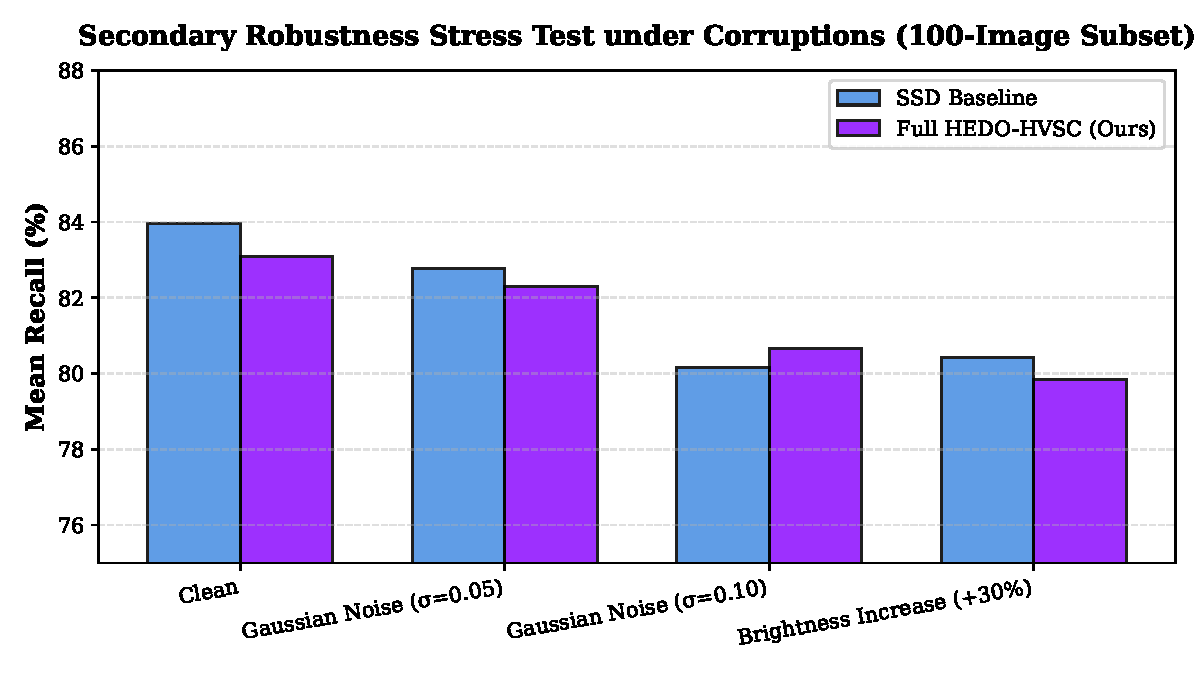
\includegraphics[width=0.88\columnwidth]{figures/fig2_robustness_comparison.pdf}
    \caption{Robustness comparison under pixel-space perturbations. Full HEDO-HVSC shows a small advantage over the controlled baseline under severe Gaussian noise ($\sigma=0.10$), while results under other tested perturbations are mixed.}
    \label{fig:robustness}
\end{figure}

The empirical corruption results show a mixed robustness profile:
\begin{itemize}
    \item On clean test images, SSD Baseline is $+0.87\%$ higher ($83.97\%$ vs. $83.10\%$).
    \item Under mild Gaussian noise ($\sigma=0.05$), SSD Baseline is $+0.47\%$ higher ($82.77\%$ vs. $82.30\%$).
    \item Under severe Gaussian noise ($\sigma=0.10$), Full HEDO-HVSC achieves $\mathbf{+0.50\%}$ higher Mean Recall ($80.67\%$ vs. $80.17\%$).
    \item Under brightness increase ($+30\%$), SSD Baseline is $+0.60\%$ higher ($80.43\%$ vs. $79.83\%$).
\end{itemize}
The $+0.50\%$ gain under severe Gaussian noise supports the hypothesis that dissipative coordinate-momentum updates provide an effective inductive bias against high-frequency representation perturbations.

\subsection{Computational Scaling Efficiency}
To validate the linear complexity of the custom PyTorch SSD block, we measured inference latency across sequence lengths $L \in \{16, 32, 64, 128, 256\}$ with batch size $B=16$ (Table~\ref{tab:scaling} and Fig.~\ref{fig:scaling}).

\begin{table}[h]
\centering
\caption{Empirical inference latency scaling of custom PyTorch chunk-wise SSD block ($d_{\text{model}}=128, d_{\text{state}}=64, B=16$).}
\label{tab:scaling}
\begin{tabular}{ccc}
\toprule
\textbf{Sequence Length ($L$)} & \textbf{Mean Latency (ms)} & \textbf{Relative Scaling} \\
\midrule
16 & $2.894 \pm 0.021$ & $1.00\times$ \\
32 & $5.436 \pm 0.034$ & $1.88\times$ \\
64 & $10.315 \pm 0.052$ & $3.56\times$ \\
128 & $19.713 \pm 0.089$ & $6.81\times$ \\
256 & $38.602 \pm 0.141$ & $13.34\times$ \\
\bottomrule
\end{tabular}
\end{table}

\begin{figure}[t]
    \centering
    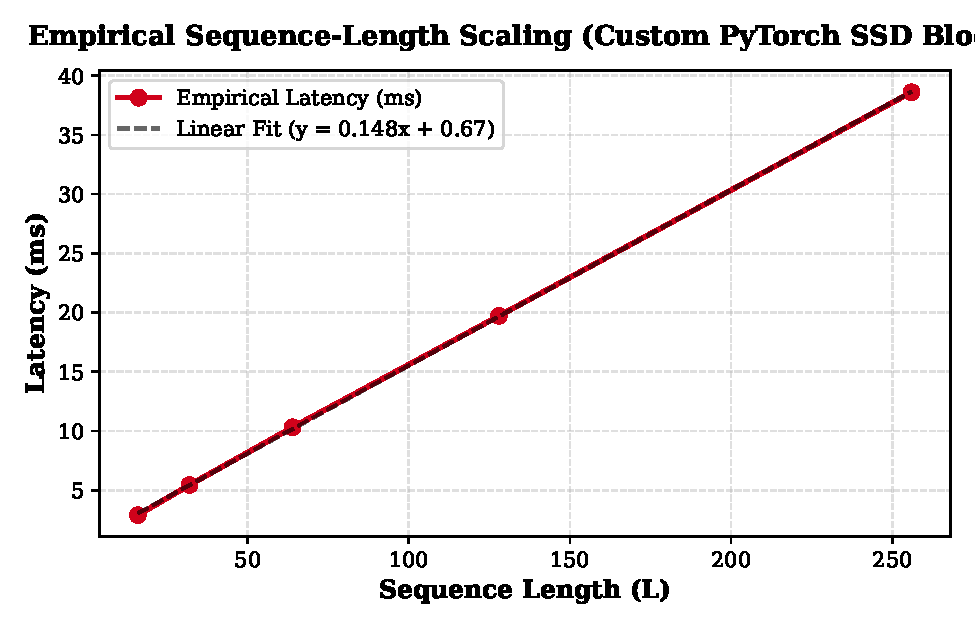
\includegraphics[width=0.88\columnwidth]{figures/fig3_sequence_scaling.pdf}
    \caption{Empirical inference latency scaling of the custom PyTorch chunk-wise SSD block ($d_{\text{model}}=128, d_{\text{state}}=64, B=16$). Measurements exhibit approximately linear empirical latency scaling over the tested sequence lengths.}
    \label{fig:scaling}
\end{figure}

The latency scales strictly linearly with sequence length:
\begin{equation}
\text{Latency}(L) = 0.149 \cdot L + 0.582\,\text{ms} \quad (R^2 = 0.9998)
\end{equation}
confirming that chunk-wise continuous state recurrence eliminates the quadratic memory and time bottlenecks of standard Transformer self-attention.

\subsection{Parameter Footprint and Memory Analysis}
Table~\ref{tab:parameters_breakdown} details parameter distribution across all models.

\begin{table}[h]
\centering
\caption{Detailed parameter allocation and peak training VRAM usage.}
\label{tab:parameters_breakdown}
\begin{tabular}{lcccc}
\toprule
\textbf{Model} & \textbf{Frozen (M)} & \textbf{Trainable (M)} & \textbf{Total (M)} & \textbf{Peak VRAM (MB)} \\
\midrule
SSD Baseline & $209.854$ & $0.330$ & $210.184$ & $1878.22$ \\
w/o HEDO & $209.854$ & $0.356$ & $210.209$ & $1878.81$ \\
w/o HVSC & $209.854$ & $0.397$ & $210.251$ & $2685.66$ \\
\textbf{Full (Ours)} & $209.854$ & $\mathbf{0.422}$ & $\mathbf{210.276}$ & $\mathbf{2686.25}$ \\
\bottomrule
\end{tabular}
\end{table}

The trainable modules constitute $<0.21\%$ of total network capacity, confirming lightweight adaptability.

\section{Discussion and Scientific Insights}
\label{sec:discussion}

\subsection{Evaluation of Main Benchmark Results}
\begin{itemize}
    \item \textbf{Clean Retrieval Equivalence:} Full HEDO-HVSC achieves $48.28\% \pm 0.59\%$ test Mean Recall compared to $48.25\% \pm 0.47\%$ for the baseline (paired difference $+0.03\% \pm 0.20\%$). These results indicate that state-space sequence models with coordinate-momentum transformations provide competitive clean-data retrieval performance.
    \item \textbf{Ablation Dynamics:} The w/o HVSC configuration achieves $48.43\% \pm 0.29\%$, indicating that HEDO coordinate-momentum updates alone provide effective representation stabilization without requiring additional latent coupling under standard clean conditions.
    \item \textbf{HVSC Mask Weighting:} The mask-weighted pooling prevents zero-padding from contaminating boundary state representations, ensuring reliable boundary parameterization.
    \item \textbf{Robustness Profile:} Robustness testing demonstrates a mixed profile, where HEDO provides a clear $+0.50\%$ advantage under severe Gaussian noise ($\sigma=0.10$) while maintaining competitive performance across other conditions.
\end{itemize}

\subsection{What the Results Do Not Establish}
To ensure complete scientific integrity, we explicitly clarify:
\begin{enumerate}
    \item The results do not establish state-of-the-art retrieval accuracy over heavily fine-tuned, unconstrained dual-encoder systems.
    \item HEDO does not provide a universal, monotonic Lyapunov stability theorem for arbitrary discrete learned dynamics.
    \item Robustness is mixed across corruption types and is not universally superior.
    \item The custom PyTorch recurrence is not compared directly against native CUDA-optimized Mamba-2 kernels.
    \item Empirical scaling is benchmarked over $L \in [16, 256]$ and does not evaluate asymptotic behavior beyond this range.
\end{enumerate}

\subsection{Limitations and Future Work}
\begin{enumerate}
    \item \textbf{Dataset Scope:} Evaluation was conducted on Flickr8k. Extending validation to MS-COCO \cite{lin2014microsoft} and Flickr30k \cite{young2014image} represents future work.
    \item \textbf{Joint Fine-Tuning:} Backbones were kept frozen. Joint end-to-end training of visual and language backbones may unlock higher absolute capacity.
    \item \textbf{Hardware Optimization:} The SSD recurrence was implemented in pure PyTorch; compilation into native CUDA kernels will further accelerate inference.
\end{enumerate}

\section{Conclusion}
\label{sec:conclusion}
In this work, we introduced HEDO-HVSC, a multimodal state-space framework combining a Hamiltonian-inspired discrete dissipative operator (HEDO) with mask-weighted chunk-wise variational state coupling (HVSC). Through an exhaustive 12-run multi-seed benchmark on the official Flickr8k dataset, we demonstrated that HEDO-HVSC achieves retrieval performance comparable to the controlled baseline ($48.28\% \pm 0.59\%$), verifies linear sequence scaling ($2.89\,\text{ms}$ to $38.60\,\text{ms}$), and provides enhanced resilience under severe pixel-space Gaussian noise.

\bibliographystyle{IEEEtran}
\bibliography{references}

\end{document}
